\section{Metodología.}

A lo largo de esta sección se detalla la metodología empleada para el desarrollo de los diferentes clasificadores. La metodología escogida sigue la filosofía del estándar de la industria CRISP-DM obviando por supuesto la fase de despliegue y puesta en producción de los modelos.

\subsection{Entendimiento del problema / negocio.}

A lo largo de esta fase se ha revisado el contenido del sitio oficial en internet de la PVA para entender bien la labor realizada por la asociación, la labor de los donantes, los diferente medios existentes para realizar donaciones, etc. 

También se ha revisado el contenido del fichero \emph{cup98doc.txt} que se encontraba disponible junto los ficheros de datos dentro de la página de descarga del KDD Contest \cite{KDD-CUP-1998} del grupo SIG-KDD (ACM) \cite{SIGKDD-ACM}, con una breve descripción del contexto del problema.

\subsection{Auditoría de datos.}

La fase de auditoría de datos ha sido la más extensa en tiempo dentro de todo el proyecto. En un primer momento se trato de realizar esta fase con la herramienta Weka \cite{WEKA} propuesta como herramienta de trabajo al comienzo del proyecto. Finalmente, tuvo que descartarse el uso de esta herramienta para esta fase, dado que presenta bastantes problemas de rendimiento y eficiencia para el trabajo con conjuntos de datos relativamente grandes. En este caso, a pesar de no contar con un conjunto de datos excesivamente grande, la herramienta Weka no conseguía desenvolverse con facilidad.

Se estudiaron diversas alternativas de trabajo para poder auditar y manipular los datos. Una de las opciones estudiada fue cargar los ficheros en tablas de un servidor de base de datos MySQL y manipularlas a través del propio lenguaje SQL. Aunque esta opción funcionaba y desde el punto de vista del rendimiento era bastante óptima, el lenguaje SQL no se mostraba como un lenguaje cómodo para el análisis estadístico.

Tras revisar que otras opciones existentes había en el mercado se opto por realizar toda la fase de auditoría y todas las fases posteriores de manipulado y preparación de la información previas a la fase de modelado con la herramienta R \cite{R}. R es un software de libre distribución para el tratamiento estadístico y la generación de gráficos por ordenador. Funciona en diversas plataformas UNIX y en el entorno Windows. Esta dotado de gran cantidad de utilidades y herramientas que facilitan el análisis estadístico y cuenta con varios plugins y módulos adicionales para trabajar con grandes cantidades de información, como por ejemplo, BigMemory.
Finalmente, no fue necesario hacer uso de ninguno de estos plugins adicionales, y con las instrucciones y herramientas básicas se pudo proceder a realizar la auditoría.

Como resultado de esta auditoría se ha construido un documento Excel maestro que contiene todas las variables y la información básica de la auditoría: 

\begin{itemize}

\item{Tipo de variable: numérica o categórica.}
\item{Número de valores distintos para las variables categóricas.}
\item{Número de valores nulos. Porcentaje de valores nulos.}
\item{Número de valores blancos. Porcentaje de valores blancos.}
\item{Valor mínimo para las variables numéricas.}
\item{Valor máximo para las variables numéricas.}
\item{Valor medio para las variables numéricas.}
\item{Valor de la mediana para las variables numéricas.}

\end{itemize}

Debido al elevado número de variables con el que se trataba y la escasa experiencia manipulando los datos con la herramienta R y la curva de aprendizaje que supuso, se decidió sólo trabajar con los conjuntos de datos de la información detallada del cliente y las variables resumen de las campañas recibidas y las donaciones realizadas.

Se decidió prescindir del detalle de las campañas de los últimos 24 meses al encontrarse esta información resumida en las variables resumen de las campañas recibidas y se decidió prescindir también de la información del censo al tratarse de información generalista y no información de carácter individual que puede ser útil para completar modelos pero no como base o punto de partida para construir un modelo.

A continuación se muestra el contenido de la hoja excel para las diferentes variables analizadas:

\begin{figure}[H]
\begin{center}
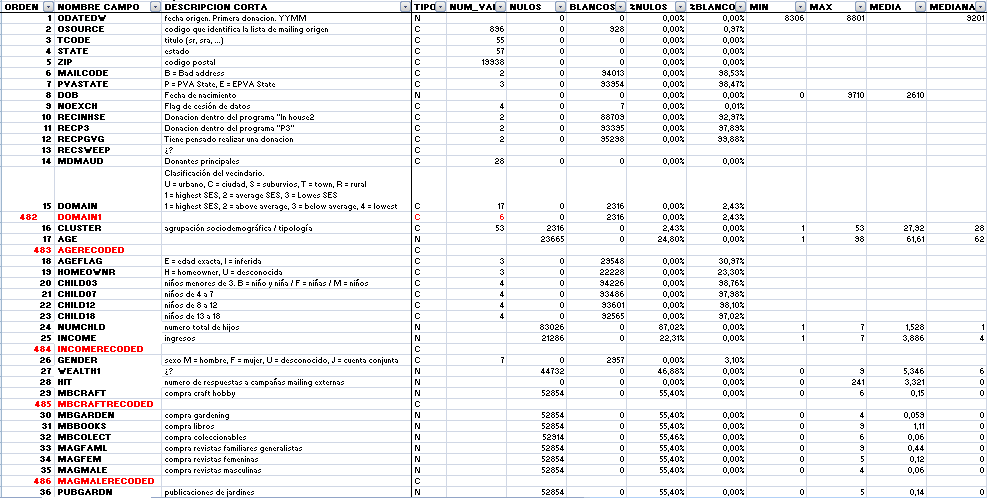
\includegraphics[width=0.95\textwidth]{img/audit1}
\caption{Captura de pantalla del excel de la auditoría de datos.}
\end{center}
\end{figure}

\begin{figure}[H]
\begin{center}
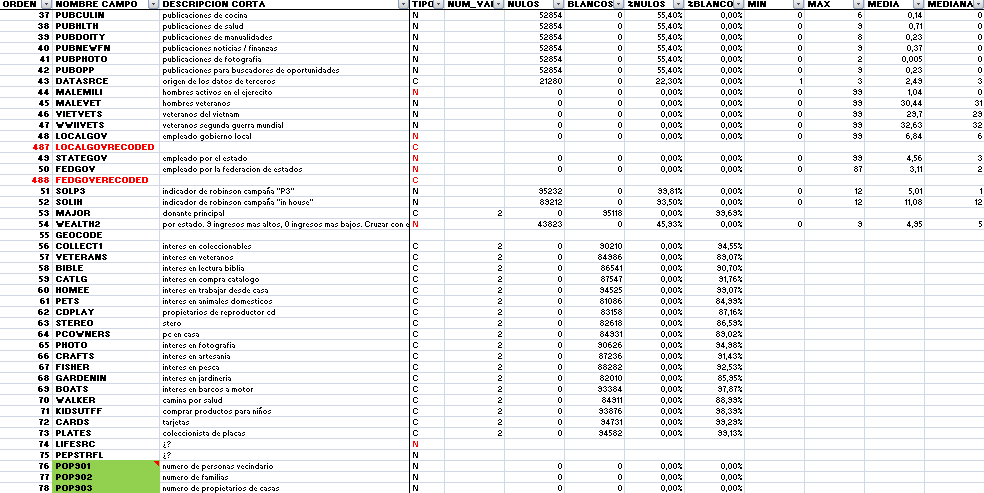
\includegraphics[width=0.95\textwidth]{img/audit2}
\caption{Captura de pantalla del excel de la auditoría de datos.}
\end{center}
\end{figure}

\begin{figure}[H]
\begin{center}
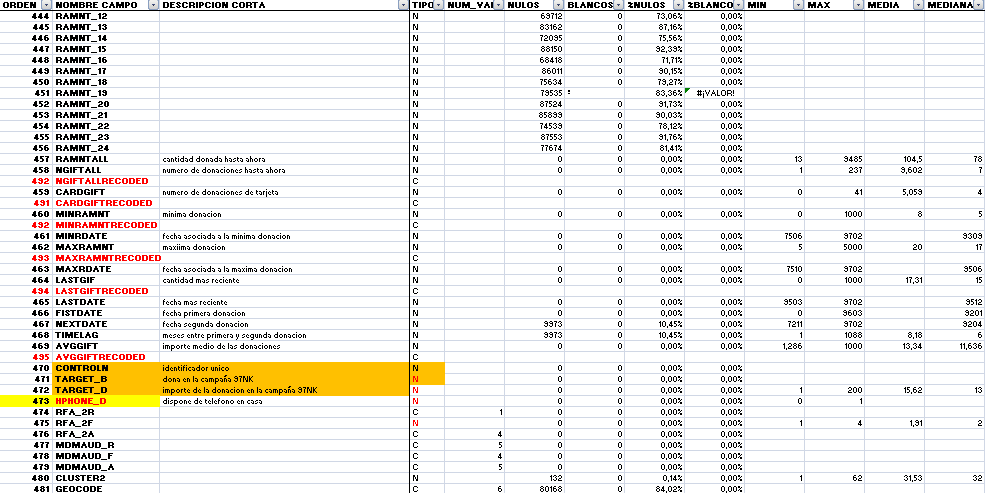
\includegraphics[width=0.95\textwidth]{img/audit3}
\caption{Captura de pantalla del excel de la auditoría de datos.}
\end{center}
\end{figure}

\subsection{Análisis univariante y recodificación de variables.}

Una vez realizada la auditoría se procedió a abordar la fase del análisis univariante donde se analiza la relación existente entre cada una de las variables de los conjuntos analizados y la variable objetivo del modelo que indica si un donante respondió positivamente al mailing enviado, realizando una donación.

Para realizar este análisis se procedió a automatizar una rutina en código R que permitiera realizar un test chi-cuadrado de cada una de las variables categóricas seleccionadas con la variable objetivo. Esta prueba permite medir el grado de asociación entre dos variables con un determinado nivel de confianza. El test se aplico de forma automática de dos formas diferentes: sin la corrección de Yates y con la corrección de Yates para seleccionar el valor adecuado del test en los casos en los que alguna combinación de valores de la variable objetivo y la variable a analizar presentan una frecuencia inferior a 5 casos.

Se completo el contenido de la hoja excel con el valor obtenido para el estadístico chi-cuadrado del test y con el p-valor asociado a este estadístico. A continuación se muestra el contenido de la hoja excel con los resultados del test:

\begin{figure}[H]
\begin{center}
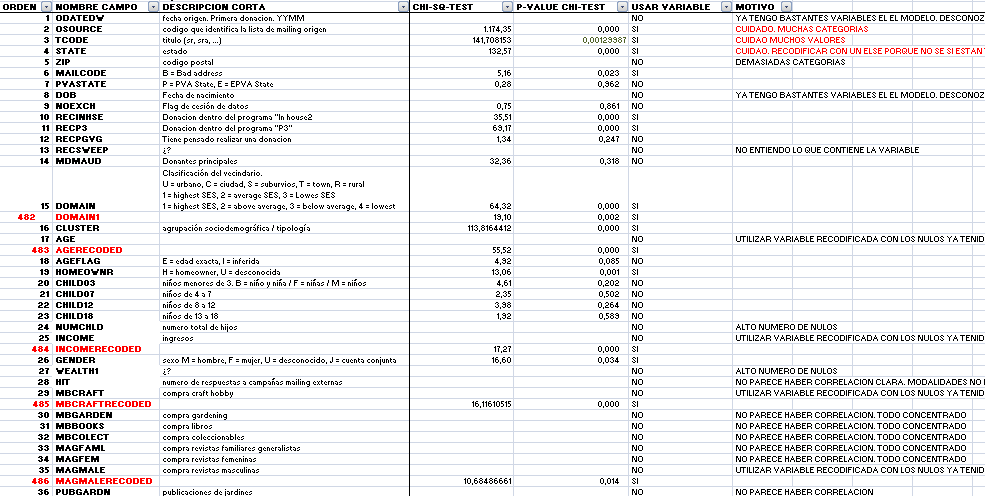
\includegraphics[width=0.95\textwidth]{img/univariante1}
\caption{Captura de pantalla del excel con los resultados del test chi-cuadrado y el p-valor asociado}
\end{center}
\end{figure}

Para las variables numéricas se procedió a automatizar una rutina en código R que partía en intervalos la variable y se analizaba el porcentaje de casos positivos de la variable target en cada uno de los intervalos. Este análisis permitía observar si el porcentaje de target era similar en todos los intervalos, de forma que no existe correlación entre la variable numérica y la variable target, o si por el contrario, según cambiabas de intervalo, el porcentaje de target era sensiblemente diferente.

\begin{figure}[H]
\begin{center}
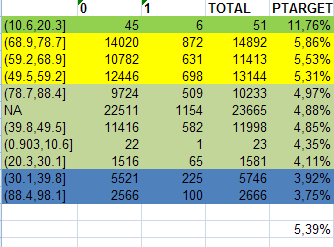
\includegraphics[width=0.4\textwidth]{img/cuantitativa1}
\caption{Captura de pantalla del excel con análisis de la correlación entre una variable numérica y la variable target}
\end{center}
\end{figure}

\begin{figure}[H]
\begin{center}
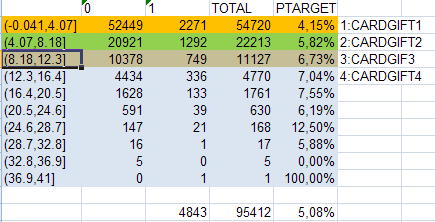
\includegraphics[width=0.4\textwidth]{img/cuantitativa2}
\caption{Captura de pantalla del excel con análisis de la correlación entre una variable numérica y la variable target}
\end{center}
\end{figure}

Con esta información se procedió a categorizar las variables numéricas que si mostraban una clara relación con la target. Sobre todo las variables que resumían el número de campañas recibidas y el número de donaciones realizadas. Sobre estas nuevas variables categóricas se volvió a realizar el test de la chi-cuadrado.

\subsection{Selección de variables.}

En la fase de selección de variables se establecieron varios criterios para limpiar la lista inicial de posibles variables candidatas y definir el conjunto final de trabajo. En concreto:

\begin{itemize}

\item{Variables con porcentaje de nulos o blancos superior al 20\%.}
\item{Valor del test de chi-cuadrado alto con un p-valor igual o inferior a 0,05.}
\item{Variable categórica con 15 o menos posibles valores diferentes. Priorizando variables con 5 valores o menos.}
\item{Variable numérico que guarda correlación con la variable target. Se incluye la variable numérica y la variable categórica recodificada.}

\end{itemize}

Las variables que contenían nulos fueron recodificadas agrupando las categorías en función del porcentaje de target y los nulos fueron agrupados con alguna de las categorías o se creo una categoría propia para ellos.

A continuación se muestra el listado final de variables seleccionado para entrenar los diferentes modelos:

\begin{figure}[H]
\begin{center}
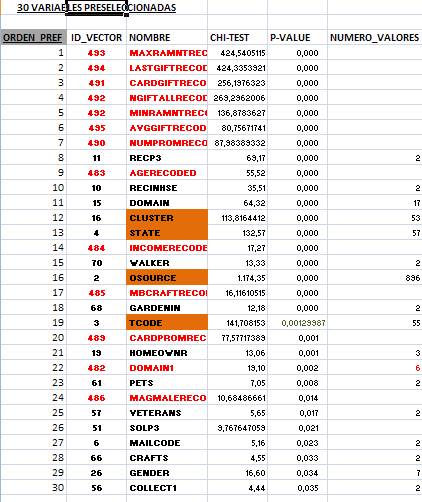
\includegraphics[width=0.7\textwidth]{img/seleccion}
\caption{Selección de variables para utilizar en la fase de modelado.}
\end{center}
\end{figure}


\subsection{Balancear ficheros de entrenamiento.}

Los conjuntos de entrenamiento y validación con las variables seleccionadas y recodificadas presentaban una gran descompensación en cuanto al número de casos positivos y casos negativos de la variable target. Esto impide que algunos algoritmos de aprendizaje, especialmente en el caso de los árboles, aprendan correctamente, favoreciendo la clasificación completa de todos los casos como casos negativos. 

Para solventar esta situación se precedió a codificar en lenguaje R una rutina de sobremuestreo que permitiera equilibrar en los ficheros de entrenamiento el número de casos positivos y negativos de la variable target.

Con esta rutina se construyo un dataset de entrenamiento con 7.770 instancias, de las cuales, 3.885 positivas y 3.885 negativas.

\subsection{Construcción de los modelos.}

La fase de construcción de los modelos ha sido ejecutada siguiendo los mismos pasos para cada uno de los algoritmos identificados como algoritmos potenciales para construir los clasificadores:

\begin{itemize}

\item{Ejecución del algoritmo con todas las variables del fichero de entrenamiento.}
\item{Ajuste de los parámetros del algoritmo y ejecución con todas las variables hasta encontrar configuración adecuada del mismo.}
\item{Ejecuciones con diferentes selecciones de variables hasta encontrar conjunto óptimo de variables, considerando óptimo, como el algoritmo que proporciona mejores resultados sobre el conjunto de entrenamiento a través de un proceso de cross validation con 10 conjuntos.}
\item{Selección de los dos o tres modelos con mejores resultados de clasificación para utilizarlos en la última etapa de validación.}

\end{itemize}

Se ha construido una hoja excel por cada algoritmo donde se puede ver la secuencia de variables utilizadas y los resultados sobre el conjunto de entrenamiento. Estas hojas están detalladas en la siguiente sección del documento.

\subsection{Validación de los modelos.}

Una vez seleccionados los dos o tres modelos con mejores resultados por algoritmo se ha contrastado la eficiencia de los mismos contra el fichero de validación para verificar que realmente no existe un sobreajuste sobre la muestra de entrenamiento y los resultados del clasificador son suficientemente estables. 

Con esta información se ha elaborado finalmente la lista de modelos potenciales para ser utilizados en las campañas reales.